% Document
\documentclass[11pt,a4paper]{article}
\usepackage[utf8]{inputenc}

% Bibliography and formatting
\usepackage[english]{babel}
\usepackage{csquotes}
\usepackage[super,comma,sort&compress]{natbib}

\usepackage{url}
\urlstyle{rm} % typeset urls in roman instead of in typewriter style
\makeatletter
\renewcommand\@biblabel[1]{#1.} %from [1] to 1
\makeatother

% Code and color
\usepackage{xcolor}

% Standard math packages etc
\usepackage{amsmath}
\usepackage{amsfonts}
\usepackage{amssymb}
\usepackage{amsthm}
\usepackage{graphicx}
\usepackage{float}
\usepackage{indentfirst}

% Package for commenting
\usepackage[colorinlistoftodos,prependcaption,textsize=tiny]{todonotes}

\oddsidemargin -10mm
\textwidth 180mm
\topmargin -10mm
\textheight 250mm

% Shortcut commands for mathbb letters
\newcommand{\N}{\mathbb{N}}
\newcommand{\Z}{\mathbb{Z}}
\newcommand{\C}{\mathbb{C}}
\newcommand{\I}{\mathbb{I}}
\newcommand{\R}{\mathbb{R}}
\newcommand{\Q}{\mathbb{Q}}

% Shortcut commands for proofs
\newtheorem{corollary}{Corollary}
\newtheorem{theorem}{Theorem}
\newtheorem{lemma}{Lemma}

\author{Alex Mirrington\\Craig Tiu\\Christian Luelf}
\title{A Comparison of Various Multinomial Classifiers on the\\MNIST Fashion Dataset}

\begin{document}
\maketitle
\tableofcontents

\pagebreak

\begin{abstract}
\noindent This report explores the potential of image-based classification techniques on real world applications. Classifiers are to be built from scratch, and performed on the Fashion-MNIST dataset. The results are then compared not only to each other, but to the official study and tests done by Fashion-MNIST. The selected classifiers to be tested and compared in this study include Linear SVM, Binary and Multinomial Logistic Regression, Naive Bayes, Nearest Neighbor, and Neural Network. Parameter tuning is performed to showcase the effect of these changes to the performance and results of the algorithms. Additionally, confusion matrices are also included to provided a deeper insight to these classifiers. The results of the study showed Nearest Neighbor and Neural Network performing the best relatively closely to each other, i.e. with highest accuracies around 85\%. These were not on par with the results from the Fashion-MNIST study which are upwards of around 95\%. However, the study concluded that further research, data collection, and better time constraints may improve the performance of the classifiers, and that this may be a step in the right direction for the highly powerful tool that is machine learning.
\end{abstract}

\pagebreak

%%%%%%%%%%%%%%%%%%%%
%%% Introduction %%%
%%%%%%%%%%%%%%%%%%%%
% - What is the aim of the study?
% - Why is the study important?
%%%%%%%%%%%%%%%%%%%%%%%%%%%%%%%%%%%
%%% Additional marking criteria %%%
%%%%%%%%%%%%%%%%%%%%%%%%%%%%%%%%%%%

%%% Presentation [8]
% - Academic style, proper grammatical sentences, no spelling mistakes
% - Good structure and layout, consistent formatting
% - Appropriate citation and referencing
% - Use charts, graphs and tables to summarise data and compare results

%%% Others [7]
% At discretion of the marker, for impressing the marker, exceeding expectation, etc. Some examples include:
% - Fast code: code runs in under 10 mins
% - High accuracy: top 10 percentile or above 85%
% - Using Latex instead of Word

%%% Code
% - Code runs and classifies within a reasonable time [10]
% - Code is well organised, easily understood with inline comments and proper documentation [10]

%%% Penalties
% - Badly written code: 
% -- Coding style and naming convention are not consistent [-10]
% -- Coding without proper use of functions or refactoring [-10]
% - Low accuracy: below 65% [-10]
% - Plagiarism: Copy source code or snippets of code from the Internet or other sources [-20]
% - Plagiarism: Copy report, article, book, journal, research paper or online resources without appropriate referencing and citation [-20]
% - Do not follow file naming rules for submission [-10]
% - Do not submit the correct files or correct number of files [-10]
% - Report exceeds more than 20 pages [-10]
% - Do not include predicted results on test examples [-10]
% - Do not include hardware and software spec used for evaluation [-10]
% - Do not include clear and detailed instructions in the report appendix on how to successfully run the code [-10]
% - Do not follow assignment instructions other than the ones already listed [-10]
% - Late submission [-20] for each day late

\section*{Introduction}
\addcontentsline{toc}{section}{Introduction}
%%%%%%%%%%%%%%%%%%%%
%%% Introduction %%%
%%%%%%%%%%%%%%%%%%%%
% - What is the aim of the study?
% - Why is the study important?

\noindent The following report is about benchmark testing on an excerpt of the Fashion-MNIST data set\cite{web:fashion_mnist} using various classifiers, implemented using limited Python libraries. The provided Fashion-MNIST dataset ensembles an alternative to the de-facto standard for classification tasks in the context of image recognition, the MNIST dataset \cite{lecun-98}.\\

\noindent This study aims to showcase the potential of image-based learning on real world applications. In particular, the predictive power of algorithms like Logistic Regression, K-Nearest Neighbor and Neural Networks are highlighted by creating classifiers for the Fashion-MNIST data set. The dataset consists of a training set of 30,000 entries and a test set of 10,000, with each entry being a 28x28 gray-scale image belonging to one of 10 classes. We are tasked to devise highly accurate classifiers to correctly classify the 10,000 test set examples with an accuracy of at least 85\% in a reasonable time (less than 10 minutes).\\

\noindent Due to the fast development in deep learning over the last years, prediction on the original MNIST dataset has increased to 99.79\% \cite{xiao2017/online}, and well above 95\% on the Fashion-MNIST dataset \cite{web:fashion_mnist}. This puts heavy pressure to classifiers - specifically those to be created from scratch in this study. Further, without the help of basic python libraries and no usage of existing implementations will prove to be a challenge in the construction of said classifiers.\\

\noindent Having said that, the conclusions regarding performance to be discussed in the latter part of this document can provide some globally-reached foresight on deep learning. Ultimately, the study could be the key to not only uncovering crucial insights about the effectiveness of chosen machine learning algorithms on image-based data, but perhaps to also pave the way to the perpetual growing world of artificial intelligence.

\pagebreak



\section*{Method}
\addcontentsline{toc}{section}{Method}
%%%%%%%%%%%%%%
%%% Method %%%
%%%%%%%%%%%%%%
% - Describe any pre-processing techniques and justify
% - Classifier: describe classifier methods/algorithms and provide reasoning for your choice and design of classifiers
\subsection*{Dataset}
\addcontentsline{toc}{subsection}{Dataset}

\noindent As mentioned previously, the data set provided to us is a subset of the Fashion-MNIST data set \cite{web:fashion_mnist}. The training set includes 30,000 examples, and the test set contains 10,000 examples. Each example is a 28x28 gray-scale image, which means a total of 784 features for each. Additionally, the classes of the first 2,000 examples from the test set are given for self validation purposes.



\subsection*{Pre-processing}
\noindent
\textbf{Stratified Folds}\\

\noindent Stratified 10-fold cross-validation was used in training classifiers. This allowed better representation of the training set as a whole, minimising risks for overfitting.\\

\noindent
\textbf{Data Shuffling}\\

\noindent Data shuffling was performed in some models such as the neural network, where it is done every epoch. Each x entry is 'zipped' with its respective y entry and shuffled. This simply ensures that the order of the given examples does not affect the training of the classifier.\\

\noindent
\textbf{Multiclass to Binary Class Conversion}\\

\noindent This method was implemented to allow the use of binary classification techniques on multinomial data. One-versus-rest or one-versus-all approach is used on each of the 10 classes, i.e. split the classes into 10 different partitions into two such that each class is separated from the rest in each partition:
\begin{itemize}
    \item takes $n$ binary classifiers, where  $n$ is the number of classes in the dataset (10 for the MNIST-Fashion dataset).
    \item The $k$th binary classifier is trained on a modified dataset, where class $c_k$ is relabelled as 0 and all other classes are relabelled as 1.
    \item Once all classifiers have been trained, new samples are predicted by  each of the $n$ classifiers, where the  $k$th classifier returns the probability that the data sample belongs to class  $c_k$. The largest of these probabilities becomes the predicted class for the sample.\\
\end{itemize}

\noindent
\textbf{PCA}\\

\noindent Principle component analysis allowed for the reduction in the number of features, while keeping a reasonable explained variance. We have found that the reduction of the number of features from 784 down to 180 significantly increased run times of the algorithms, while keeping core features responsible for 98\% of explained variance.\\

\subsection*{Classifiers}
\addcontentsline{toc}{subsection}{Classifiers}

% - This part has to be shifted to the Method!
\noindent
\textbf{Linear SVM}\\

\noindent The linear support vector machine is one of the six implemented models for this study. Its objective includes finding a N-dimensional hyperplane with optimal/maximum margin. Specifically, one in a 2-dimensional space for a linear one.\\

\noindent Since this is a binary classifier, the conversion method mentioned earlier was used to gather meaningful results from the multinomial dataset (one-versus-rest approach).\\

\noindent Having said that, the runtimes of support vector machines are notoriously slow, taking upwards of 50 hours on some studies. This is because the algorithm is known to have big-O close to O(n\textsuperscript{3}). Our implementation had training time of 30 minutes for each epoch, rendering it unusable, and thus not included in the final report.\\

\noindent
\textbf{Binary Logistic Regression}\\

\noindent Another binary classification method is binary logistic regression. The difference between this one and the previous is that probabilities are first considered before predicting a class. That is, the probability that the given features belong to the class versus the probability that it doesn't belong to the class. Since probabilities are considered, a sigmoid activation function is needed and used to output $\in [0, 1]$.\\

\noindent Furthermore, mini-batch gradient descent, which is a variation of gradient descent, is implemented in this particular algorithm to potentially minimise cross-entropy error function. Having said that, one problem to note is that it introduces an extra hyperparameter (the batch size) for the algorithm, and can prove to be more tedious to account for it.\\

\noindent As it is another binary classifier, the one-versus-rest conversion function explained previously was used to gather useful results for the Fashion-MNIST dataset.\\

\noindent
\textbf{Multinomial Logistic Regression}\\

\noindent Following binary logistic regression, multinomial logistic regression was also implemented. This generalizes logistic regression to multinomial classification tasks, which is suitable for the given dataset. The algorithm calculates probabilities for each of the 10 classes in this case, and selecting the best class from those results.\\

\noindent Mini-batch gradient descent is also implemented for this algorithm for the same reasons described in the subsection for binary logistic regression. Since this is a multiclass classifier, softmax activation function was used instead. Also, because of this, one-versus-rest is no longer required for this algorithm as it doesn't produce binary results.\\

\noindent
\textbf{Naive Bayes}\\

\noindent A standard implementation of Naive Bayes is included in this study. The lazy learning algorithm returns the maximum log likelihood across all classes for a new sample, and assumes independence between all the features. Being a lazy learning algorithm allows the simple storing of data while training, then pushing all calculation processing strain onto the classification step.\\

\noindent Further, Laplace correction is included in this algorithm for regularisation, preventing special cases where the Naive Bayes calculation would normally yield zero. This value is included as a hyperparameter, and can be tuned as shown in the following sections.\\

\noindent
\textbf{Nearest Neighbor}\\

\noindent The K-nearest neighbor algorithm was implemented, another 'lazy' classification algorithm. A standard implementation is included, which by definition considers only the k closest data points from training. The algorithm allows for multiple distance functions:\\

\begin{itemize}
    \item Manhattan distance
    \item Euclidean distance
    \item Squared Euclidean distance (removes expensive sqrt calculations)
    \item Minkowski distance\\
\end{itemize}

\noindent
\textbf{Neural Network}\\

\noindent Finally, a neural network algorithm is also implemented for this study. The classifier also includes mini-batch gradient descent (minimising squared error), batch size hyperparameter, and multiple activation functions:
\begin{itemize}
    \item Sigmoid
    \item Tanh
    \item Relu
    \item Softplus\\
\end{itemize}

\noindent The sigmoid and softplus activations functions were successfully implemented and used in the performance of the classifiers but the implementations for tanh and relu produced errors; relu was unstable due to some possible implementation errors, and tanh converged too slowly, capping at around 70\% accuracy in initial tests.\\

\noindent A batch size of 64 has been found to be optimal due to the vectorisation of the CPU; a 32 batch size is too small and triples computation time. Greater than 64 is also feasible, but leads to getting stuck in local minima more easily.\\

\noindent
\textbf{Justifications}\\

\noindent The classifiers selected for this study cover a wide range of different classification techniques. Linear SVM and Binary Logistic Regression are chosen to test the effectiveness of binary classifiers on multinomial image datasets. Naive Bayes and Nearest Neighbors are simple algorithms that have proven to be effective time and time again. The Neural Network is a more complex algorithm shown to be effective on image datasets, particularly on the Fashion-MNIST dataset as highlighted in an official study from Fashion-MNIST.\\

\noindent
\textbf{Metrics}\\

\noindent
Metrics gathered include:
\begin{itemize}
    \item Accuracy
    \item Confusion matrix
    \item Precision
    \item Recall
    \item F1
\end{itemize}



\pagebreak

\section*{Experiments and Results}
\addcontentsline{toc}{section}{Experiments and Results}
%%%%%%%%%%%%%%%%%%%%%%%%%%%%%%%
%%% Experiments and Results %%%
%%%%%%%%%%%%%%%%%%%%%%%%%%%%%%%
% - Describe the experiments and results including accuracy and performance
% - Extensive analysis based on the following:
% -- Comparison of results between classification methods
% -- Comparison of the effect of fine tuning classifier parameters
\subsection*{Hardware and Software Specifications}
\addcontentsline{toc}{subsection}{Hardware and Software Specifications}
\noindent All results were collected on a 2017 13-inch MacBook Pro with the following specifications:
\begin{quote}
\begin{flushleft}
\begin{verbatim}
OS: macOS Mojave 10.14.6 (18G95)
CPU: Intel i5-7360U, 4 cores @ 2.30GHz 
GPU: Intel Iris Plus Graphics 640 
RAM: 8192MiB LPDDR3 @ 2133MHz 
Disk: 128GB SSD
\end{verbatim}
\end{flushleft}
\end{quote}
The notebook used Python 3.7.4, with the following modules:
\begin{quote}
\begin{flushleft}
\begin{verbatim}
h5py==2.9.0
matplotlib==3.1.1
numpy==1.17.0
pandas==0.25.1
scipy==1.3.1
\end{verbatim}
\end{flushleft}
\end{quote}

\subsection*{Classifier Parameter Tuning}
\addcontentsline{toc}{subsection}{Classifier Parameter Tuning}
\noindent To obtain a brief understanding of which classifier parameters might yield the best results, each classifier was trained on a stratified sample of the training set ($90\%$), and validated on the remainder ($10\%$). This sample was the first of the ten stratified folds used to evaluate the models after parameter tuning.\\

\noindent Ideally, all hyperparameters would be optimised simultaneously, but this was not feasible even despite the reasonably fast running time of the implemented classifiers; Optimising just 3 parameters across 10 values each involves training $10^3$ models, each of which can take up to 5 minutes each. As a result, the general approach taken towards fine tuning parameters was to optimise each parameter in turn, starting with the parameters that had the most effect on the accuracy of the model or those that were depended upon by other parameters; For the Linear Regression classifier, for example, the learning rate, $\eta$ was optimised first, since the number of epochs to train for was dependent on the selection of the learning rate.\\

\noindent A batch size of 64 was chosen for both Logistic Regression models and the Neural Network, as preliminary tests showed that a batch size of 32 tripled the running time per batch. This is due to the architecture of the CPU that the models were trained on, and the vectorised operations used by the Numpy library. Decreasing the batch size further reduced the running time per batch, but increased the running time per epoch, and led to much noisier accuracy curves on the training set. A batch size larger than 64 was not chosen, as this limited the ability for algorithms to escape local minima during optimisation.\\

\subsubsection*{Linear Regression (One vs Rest)}
\addcontentsline{toc}{subsubsection}{Linear Regression (One vs Rest)}

\noindent\textbf{Learning Rate Tuning}\\
The first parameter to be determined was the learning rate of the model, $\eta$. From preliminary tests, it was known that each Binary Logistic Regression classifier achieved a reasonable accuracy after 50 epochs, so the epoch count was set to 50 during the tuning of the learning rate. Each of the 10 binary classifiers in the one-vs-rest model (one for each label in the dataset) had a sigmoid activation function and were trained with a batch size of 64. Ten learning rates were evaluated, and metrics collected, as shown in Figure \ref{fig:logistic_regression_eta_tuning} below.

\begin{figure}[H]
    \centering
    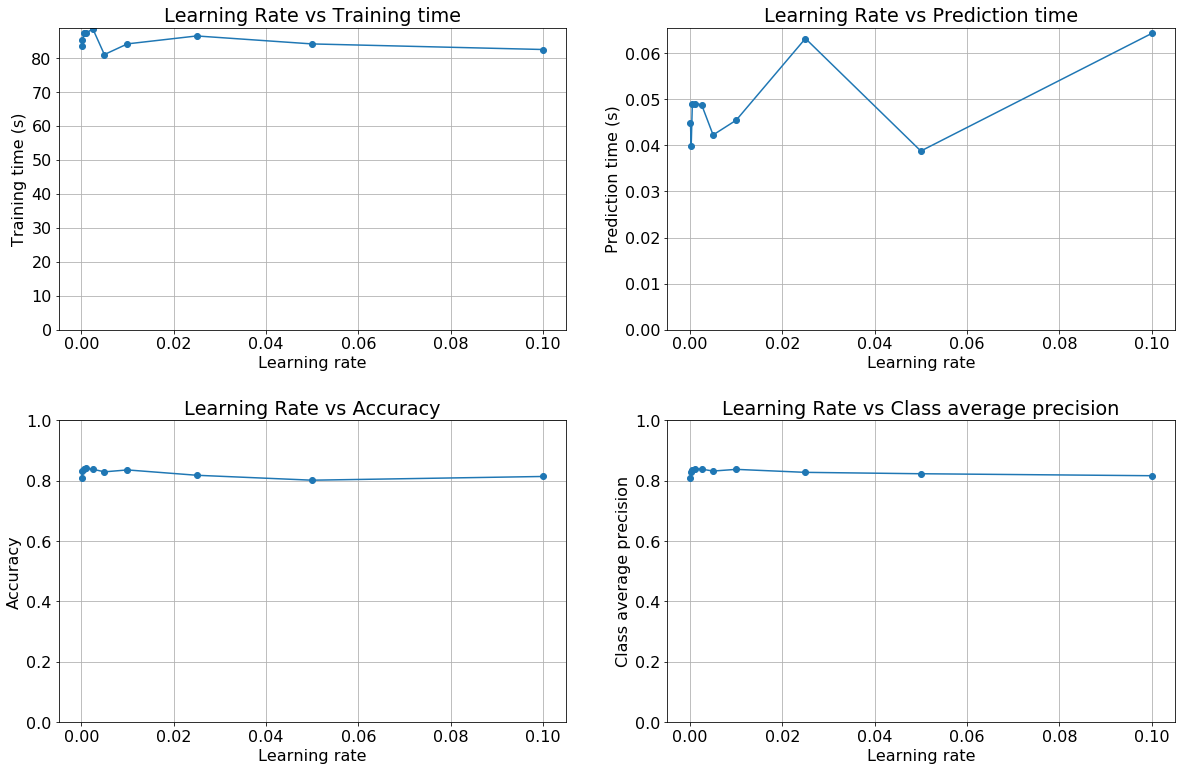
\includegraphics[width=0.9\textwidth]{img/lr_eta_test.png}
    \caption{Learning rate versus various metrics for the One-vs-Rest Logistic Regression classifier with 50 epochs per binary classifier, 64 sample batch size and sigmoid activation.}
    \label{fig:logistic_regression_eta_tuning}
\end{figure}

\noindent From Figure \ref{fig:logistic_regression_eta_tuning}, it is evident that $\eta = 0.001$ had the highest accuracy and precision. The Recall and F1 plots were not shown for sake of brevity, however these were also maximised when $\eta = 0.001$. The $\eta = 0.001$ model took the longest to train out of all the models compared in this test, however only took 10 seconds more than the fastest model. Moreover, prediction times for all models were extremely fast, at under 0.1s. Consequently, $\eta = 0.001$ was deemed to be the final learning rate to use for this classifier.\\

\noindent\textbf{Epochs}\\
Once $\eta$ had been determined, it was important to know how many epochs to train the model for. The one-versus-rest ensemble draws its results from $n$ binary classifiers, where $n$ is the number of classes in the dataset, so the best way to determine an appropriate number of epochs was to investigate when the accuracy of each of these binary classifiers ceased to improve.\\

\noindent Ten binary classifiers were trained on the same stratified sample of the training set, modified so that the $k$th classifier was trained on a set where class $c_k$ was mapped to $0$ and all other classes were mapped to $1$. Each classifier had a learning rate of $0.001$, a sigmoid activation function, and used the mini-batch gradient descent algorithm for optimisation with batch sizes of 64.\\

\noindent The best classifier reached an accuracy of $99.33\%$ on the validation set after 100 epochs, and the worst reached only $91.50\%$. (See Figure \ref{fig:worst_lr_binary_classifier_100_epochs}), however all classifiers stopped improving on the test set after around 50 epochs. The full results of this test can be found in the submitted notebook. Since all classifiers stopped improving on the test set after around 50 epochs, it is evident that the one-vs-all classifier would not gain any additional information by training each of its binary logistic regression classifier for more than 50 epochs.\\

\begin{figure}[H]
    \centering
    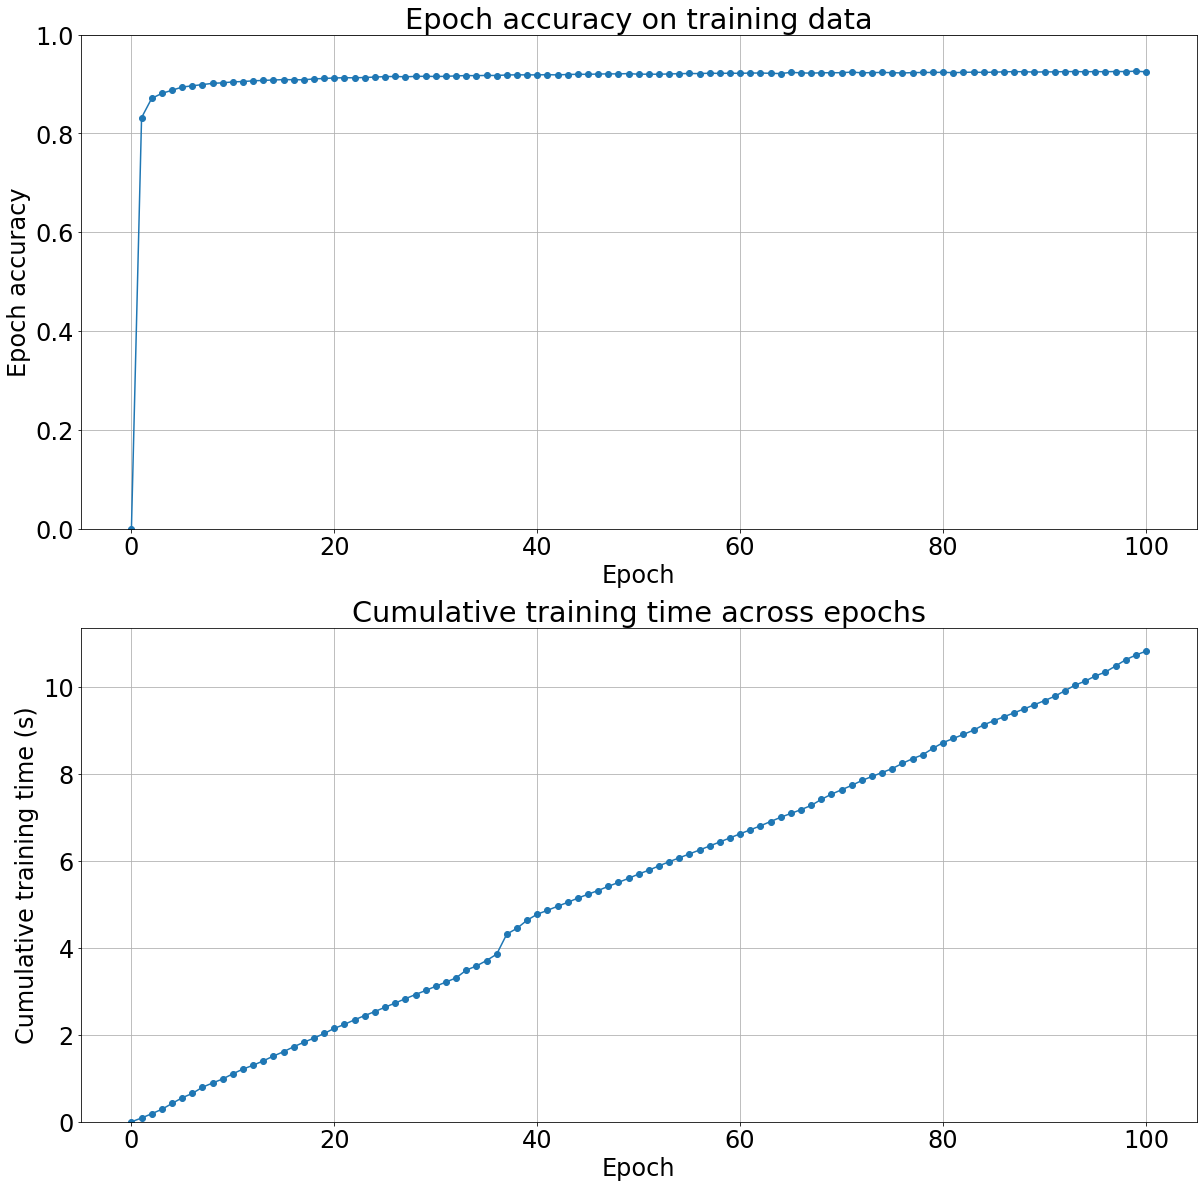
\includegraphics[width=0.9\textwidth]{img/worst_lr_epoch_test.png}
    \caption{Training set accuracy and training time across 100 epochs for a Binary Logistic Regression classifier classifying Shirts vs Non-Shirt samples.}
    \label{fig:worst_lr_binary_classifier_100_epochs}
\end{figure}

\noindent\textbf{Final Parameters}
\begin{verbatim}
eta=0.001
activation=sigmoid
batch_size=64
epochs=50
\end{verbatim}

\pagebreak

\subsubsection*{Multinomial Linear Regression}
\addcontentsline{toc}{subsubsection}{Multinomial Linear Regression}

\noindent\textbf{Learning Rate}\\
Again the learning rate was the first parameter to be optimised for the Multinomial Linear Regression classifier, since the number of epochs is dependent upon the learning rate.\\

\noindent Each classifier was run for 250 epochs, with a batch size of 64, and 10 learning rates were evaluated:\\
0.1, 0.05, 0.025, 0.01, 0.005, 0.0025, 0.001, 0.0005, 0.00025 and 0.0001\\

\begin{figure}[H]
    \centering
    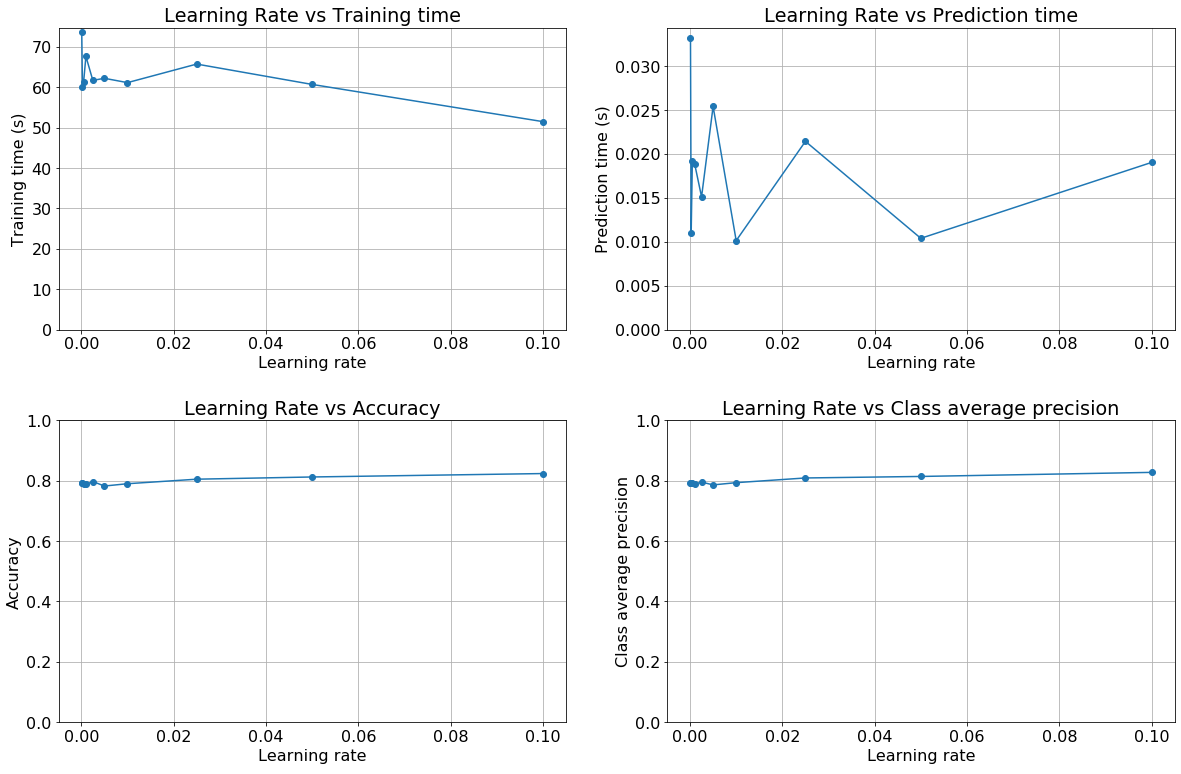
\includegraphics[width=0.9\textwidth]{img/mlr_eta_test.png}
    \caption{Learning rate versus various metrics for the Multinomial Logistic Regression classifier with 250 epochs and 64 sample batch size}
    \label{fig:multinomial_logistic_regression_eta_tuning}
\end{figure}

\noindent After examining the results as shown in Figure \ref{fig:multinomial_logistic_regression_eta_tuning}, a learning rate $\eta = 0.1$ was initiallychosen, since it had the close to the best accuracy, precision, recall and F1 of all learning rates in the test, as well as an extremely fast prediction time and reasonable training time.\\

\noindent It was also noted that the accuracy, precision, recall and f1 graphs had a slight updawrds trend as $\eta$ increased, so a few larger learning rates were tested separately on the same dataset. These additional tests showed that learning rates of 0.1 or exhibited large instability, leading to math overflow errors that could often ruin the classifier's learned parameters. It was then decided that a learning rate of $\eta = 0.05$ was more fitting than $0.1$, due to stability concerns.\\

\noindent \textbf{Epochs}\\
Upon investigating the accuracy on the training data across 250 epochs, it became evident that the multinomial logistic regression classifier was not learning much new data after around 150 epochs, however the accuracy curve was noisy, as seen in Figure \ref{fig:mlr_epoch_test} below.\\
    
\begin{figure}[H]
    \centering
    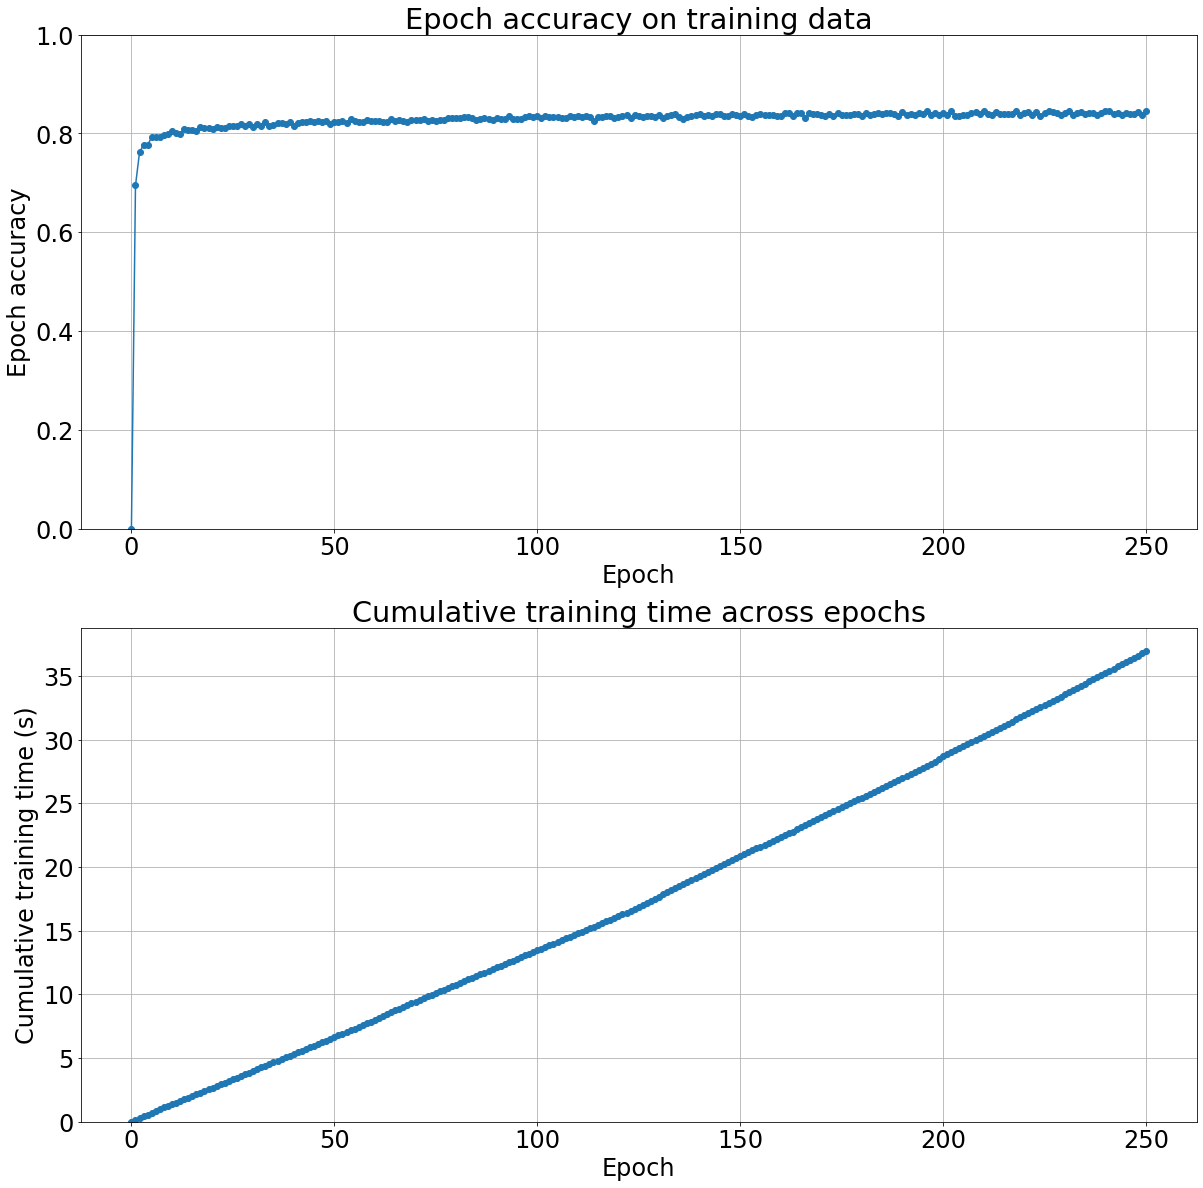
\includegraphics[width=0.9\textwidth]{img/mlr_epoch_test.png}
    \caption{Training set accuracy and training time across 250 epochs for the Multinomial Logistic Regression classifier with 64 sample batch size}
    \label{fig:mlr_epoch_test}
\end{figure}

\noindent It was decided that because the accuracy curve was so noisy, it made more sense to train the classifier for longer, to ensure that any noise has ample time to settle. Additionally, the cumulative training time curve showed that not much extra time was required to predict 250 epochs instead of 150.\\

\noindent \textbf{Final Parameters}
\begin{verbatim}
eta=0.05
batch_size=64
epochs=250
\end{verbatim}

\pagebreak

\subsubsection*{Naive Bayes}
\addcontentsline{toc}{subsubsection}{Naive Bayes}

\noindent There was no need to tune hyperparameters for Naive Bayes, since it is deterministic for a given training set; The only parameter that was used for Naive Bayes is a Laplacian smoothing parameter, used to avoid zero posterior probabilities. This parameter needs to be as small as possible but still nonzero, so as not to skew the posterior probabilities and thus the per-class probabilities of predicted samples. The Laplacian smoothing parameter was set to 1 for all trained Naive Bayes models.\\

\noindent \textbf{Final Parameters}
\begin{verbatim}
laplace=1.0
\end{verbatim}

\subsubsection*{K-Nearest Neighbour}
\addcontentsline{toc}{subsubsection}{K-Nearest Neighbour}

\noindent During preliminary tests, it was found that a $k$ value of 5 worked reasonable well for the nearest neighbour classifier, so this value was used when determining which distance function to use. The accuracies, training times and prediction times of three different distance functions were compared, as summarised in Table \ref{table:knn_dist_funcs}.

\begin{table}[H]
\centering
\begin{tabular}{|c|c c c|} 
\hline
Distance Function & Training Time (s) & Prediction Time (s) & Validation Set Accuracy \\ [0.5ex] 
\hline
Manhattan & 0.0028 & 140.1298 & 0.843 \\ 
Squared Euclidean & 0.0005 & 163.8103 & 0.838 \\
Euclidean & 0.0004 & 181.5002 & 0.838 \\ [1ex] 
\hline
\end{tabular}
\caption{Training time, prediction time, and accuracy for different distance functions on a 5-Nearest Neighbour classifier}
\label{table:knn_dist_funcs}
\end{table}

\noindent The first notable point in the data is that the validation set accuracy of the euclidean distance function and the euclidean squared distance function is the same, but the prediction time for the latter is 20s less. This is because the euclidean squared function does not need to compute expensive square roots, and $f(x) = \sqrt(x)$ is a monotonic increasing function.\\

\noindent It was however surprising that the manhattan distance had a higher accuracy on the validation set than the euclidean distance functions, in addition to its smaller prediction time. The manhattan distance function was thus chosen for the final classifier.\\

\noindent Different values for $k$ were then tested using the manhattan distance function, as shown in Figure \ref{fig:knn_k_tuning} below:

\begin{figure}[H]
    \centering
    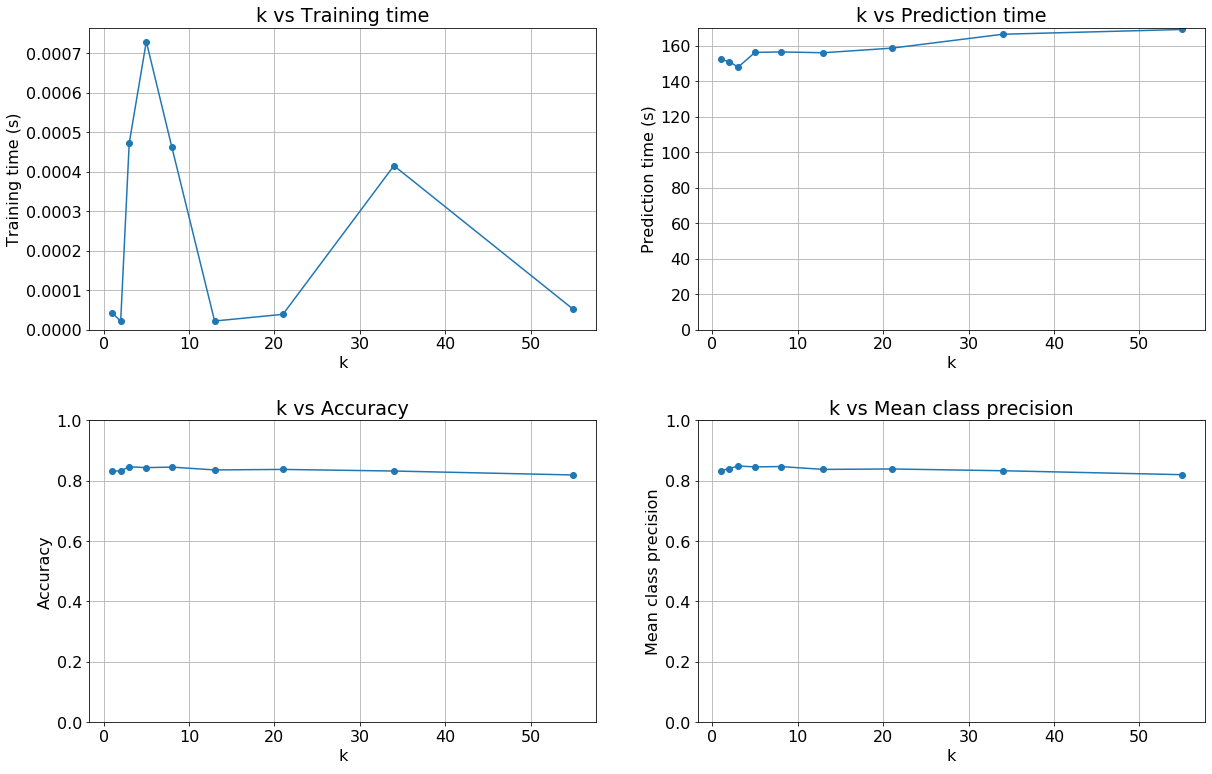
\includegraphics[width=0.6\textwidth]{img/knn_k_test.png}
    \caption{Hyperparameter $k$ versus various metrics for the K-Nearest Neighbour classifier with Manhattan distance function.}
    \label{fig:knn_k_tuning}
\end{figure}

\noindent $k=3$ was found to be the best candidate here, due to its low prediction time and high accuracy, precision, recall and F1 on validation set. Again, recall and F1 statistics were not shown for sake of brevity.\\

\noindent \textbf{Final Parameters}
\begin{verbatim}
k=3
dist=manhattan
\end{verbatim}

\subsubsection*{Neural Network}
\addcontentsline{toc}{subsubsection}{Neural Network}
\noindent \textbf{Layer Structure}\\
\noindent The neural network was the most complex model that was tested, and as such optimising its hyperparameters was much more involved. The first parameter to investigate was the layer structure and types of layers. The network was implemented with the plan of being able to use dropout, relu and pooling layers, however time constraints only allowed for the implementation of fully-connected layers.\\

\noindent Four different layer structures were investigated, each of which had their own pitfalls. All layers were fully connected, with sigmoid activations and the model was trained using a batch size of 64 and learning rate of 0.1. Tanh and relu activations were not used, as they proved instable in initial testing, most likely due to an implementation error, since others have seen better results using these activation functions over the sigmoid function \cite{xiao2017/online}.

\begin{table}[H]
\centering
\begin{tabular}{|c|c c c|} 
\hline
Layer Structure & Training Time (s) & Prediction Time (s) & Validation Set Accuracy \\ [0.5ex] 
\hline
(784, 10, 10) & 176.8052 & 0.0498 & 0.831 \\ 
(784, 100, 10) & 245.4560 & 0.0583 & 0.836 \\
(784, 100, 10, 10) & 325.6396 & 0.0525 & 0.836\\
(784, 100, 20, 10) & 347.0850 & 0.0583 & 0.848 \\ [1ex] 
\hline
\end{tabular}
\caption{Training time, prediction time, and accuracy for different layer structures.}
\label{table:nn_sigmoid_layer_structure}
\end{table}

\noindent The 3-layer structures had lower accuracies, and investigating their accuracy curves on the training set showed that they were easily getting stuck in local minima, as shown in Figure below:

\begin{figure}[H]
    \centering
    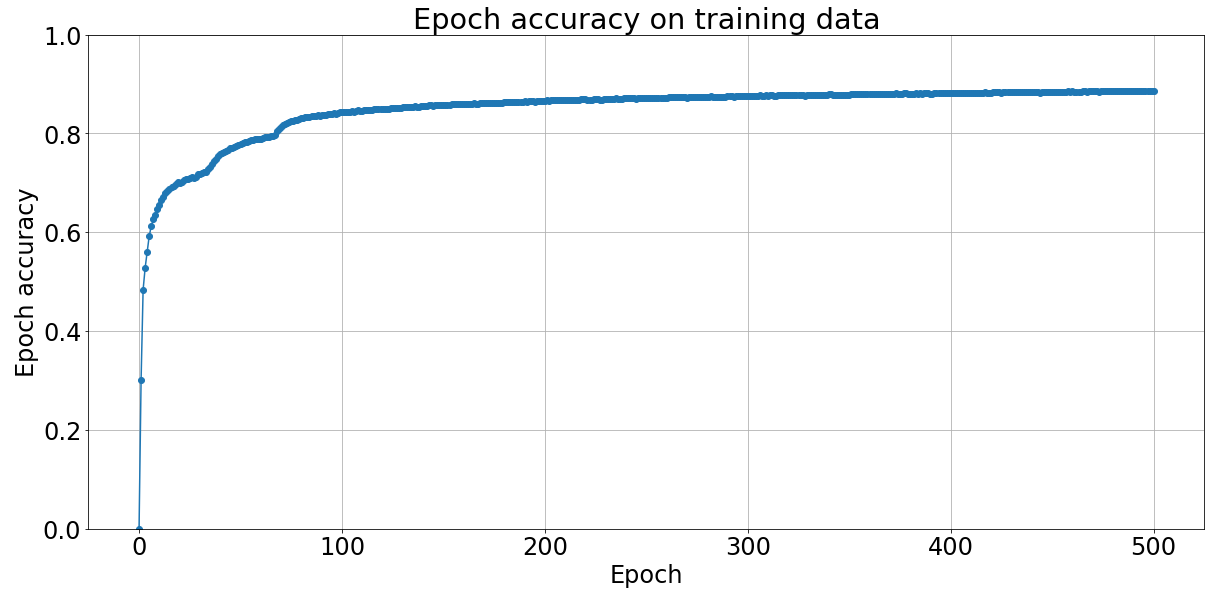
\includegraphics[width=0.6\textwidth]{img/local_minima.png}
    \caption{Accuracy on the training set for a Neural network classifier with layer structure (784, 10, 10) and sigmoid activations over 500 epochs.}
    \label{fig:nn_local_minima}
\end{figure}

\noindent The 4-layer structures had higher accuracies, though tended to overfit, having accuracies on the training data of around $95\%$, and only $85\%$ on the validation set, as shown in Figure \ref{fig:nn_784_100_20_10_overfit} below:

\begin{figure}[H]
    \centering
    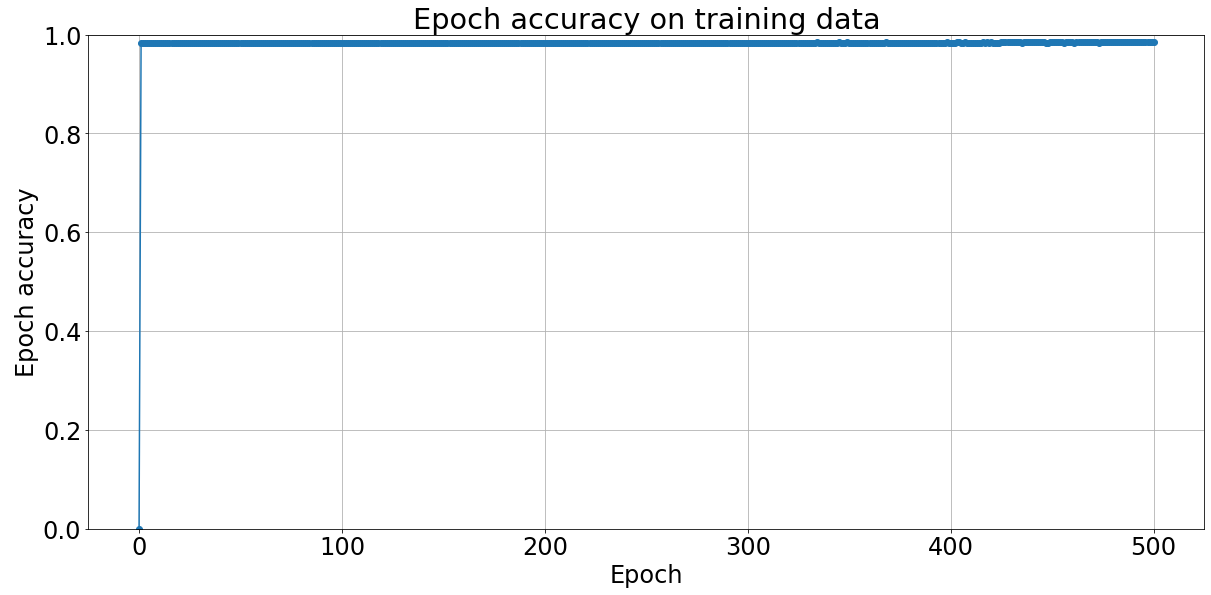
\includegraphics[width=0.9\textwidth]{img/nn_784_100_20_10_overfit_eta_0025.png}
    \caption{Accuracy on the training set for a densely-connected Neural Network classifier with a (784, 100, 20, 10) layer structure and sigmoid activation over 500 epochs with a batch size of 64 and learning rate of 0.025}
    \label{fig:nn_784_100_20_10_overfit}
\end{figure}

\noindent Overall, it was decided that a structure of (784, 100, 20, 10) was the best to use, despite overfitting, since it was less prone to getting stuck in local minima.

\noindent Similarly to other models, the learning rate was also investigated, and it was concluded that a learning rate of $\eta=0.05$ was most appropriate.\\

\noindent \textbf{Final Parameters}
\begin{verbatim}
eta=0.05
batch_size=64
epochs=250
activation=sigmoid
\end{verbatim}

\pagebreak

\section*{Discussion and Classifier Comparison}
\addcontentsline{toc}{section}{Discussion and Classifier Comparison}
%%%%%%%%%%%%%%%%%%
%%% Discussion %%%
%%%%%%%%%%%%%%%%%%
% - Produce meaningful discussion of results from the experiment and choice of classifier methods
% - Provide relevant personal reflection
\noindent Except the naive bayes classifier, the self-implemented models could achieve results on the same level of more than 80\% accuracy on the validation set. In order to further improve the accuracy, it has to be understood which errors were made during the classification. For this purpose, the confusion matrices of each classifier are evaluated. By looking at the confusion matrix of each classifier, it can be analyzed which classes caused the highest misclassification in the data (see Appendix). As expected the majority of the errors were made between classes which are closely related (e.g. by belonging to the same upper class). For example, that means that the model is able to recognize that the sample belongs to the upper class shoe but is not sure whether it is a 'Sneaker', 'Sandal' or 'Ankle boot'. The same is applicable for the classes for 'T-shirt/Top', 'Pullover', 'Coat', 'Shirt' or 'Dress' which can be considered as clothing for the upper body part. The lowest confidence existed when the classifiers predicted the class 'Shirt'. Here, the variation of the actual class is the highest (see Figure \ref{fig:accuracy}). On the other site, the highest confidence for prediction was given for the class 'Trouser'.\\
\begin{figure}[H]
    \centering
    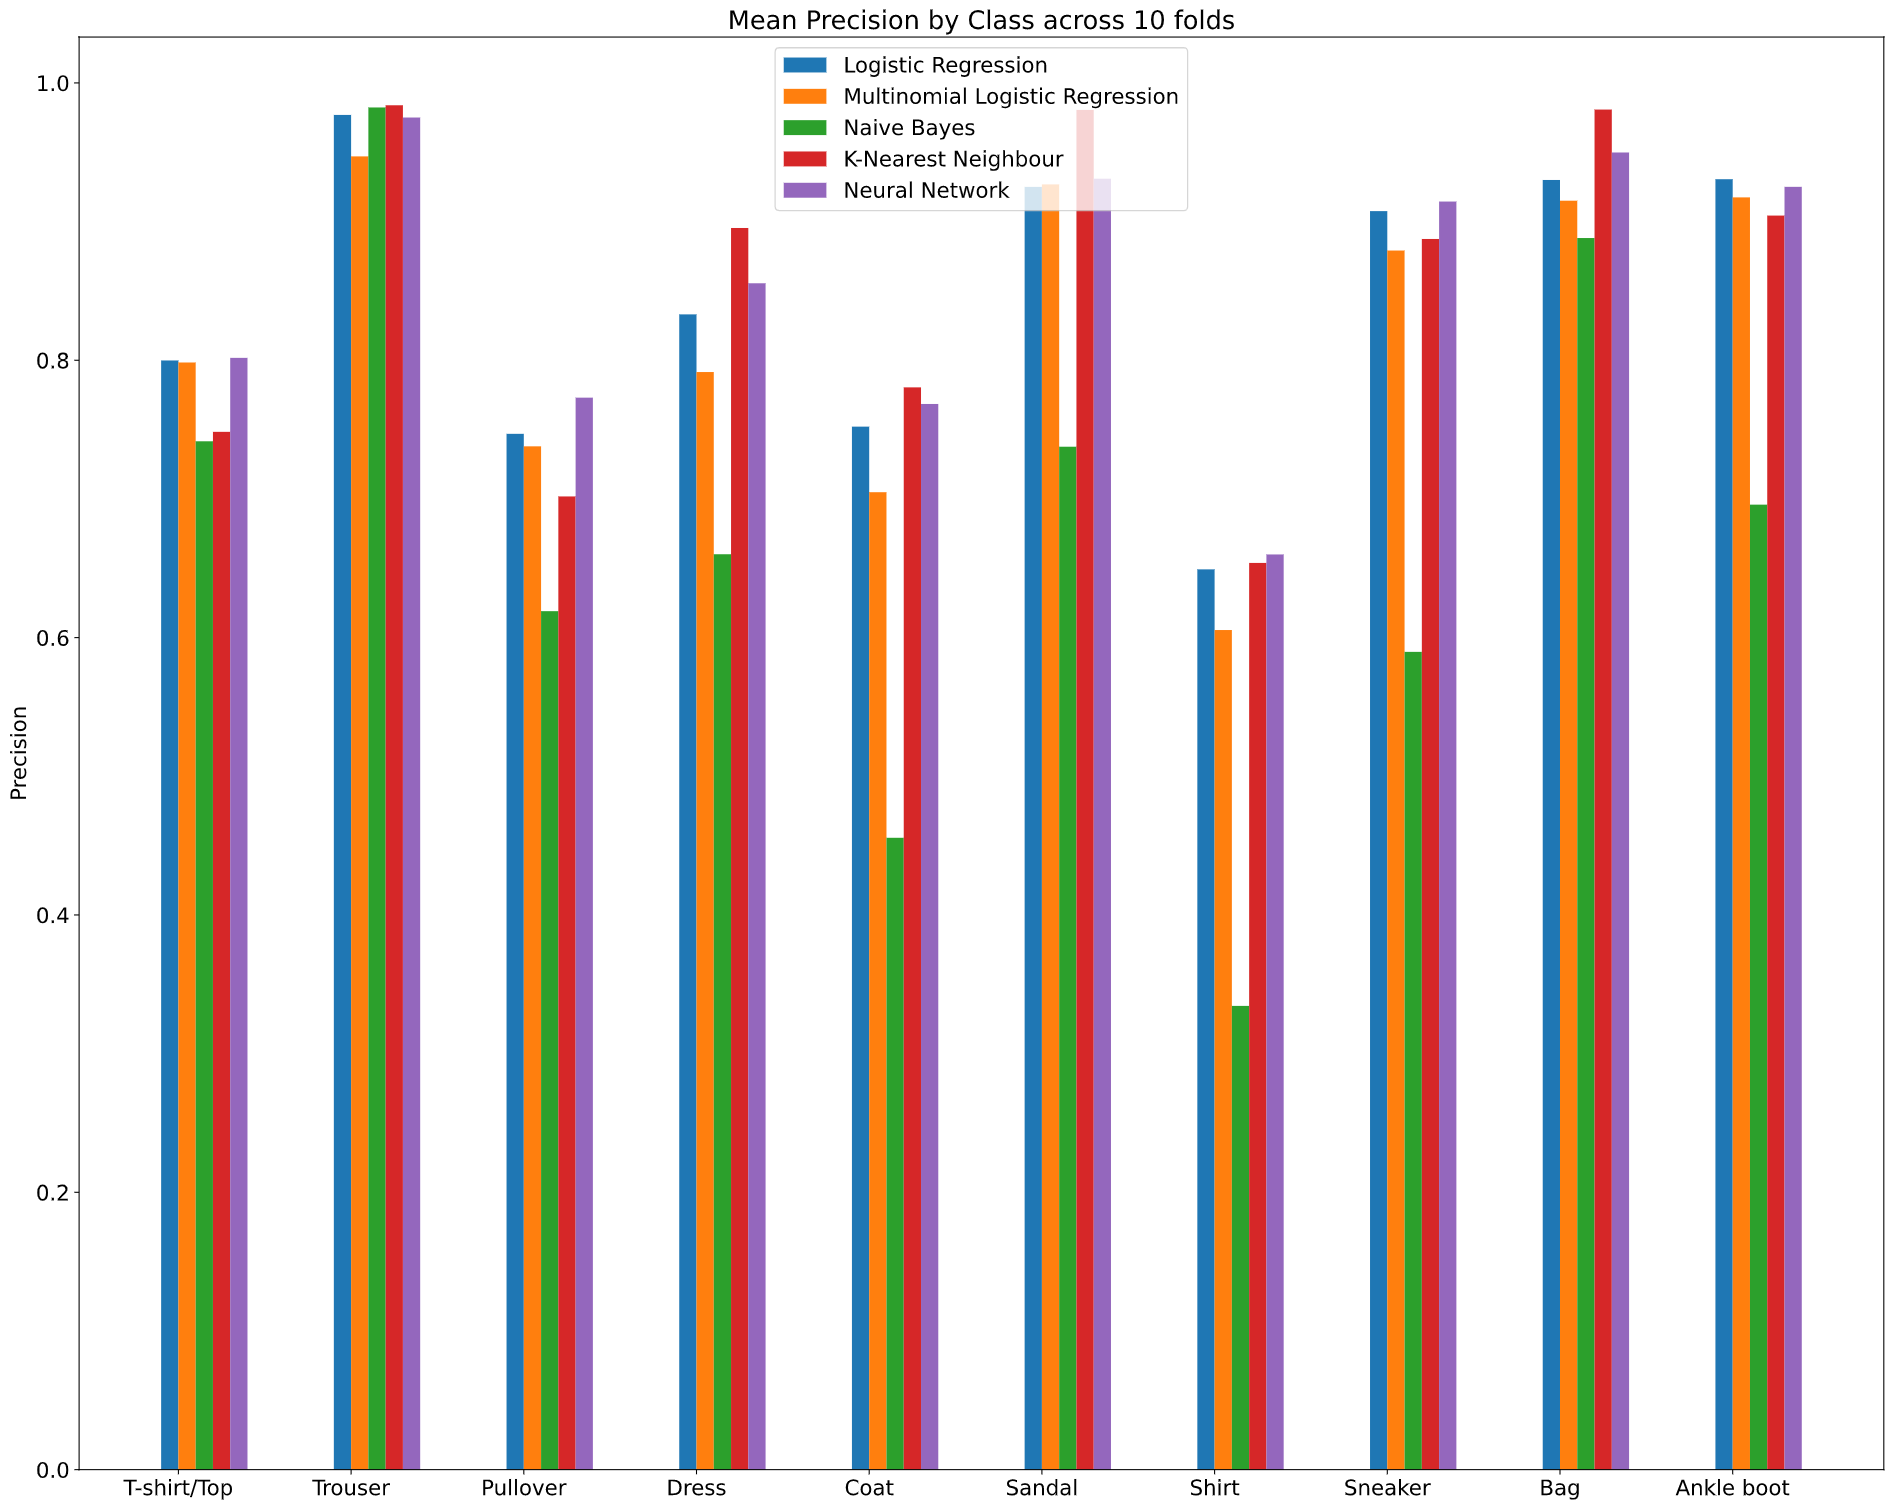
\includegraphics[width=0.9\textwidth]{img/precision_comparison.png}
    \caption{Precision for each class and classifier.}
    \label{fig:accuracy}
\end{figure}
\noindent In the next steps the final results of the five selected classifiers are evaluated in more detail and compared to published benchmark tests on the Fashion-MNIST dataset. For the comparison the results of Xiao, Rasul, Vollgraf (2017) and the Github repository of the dataset were considered.\cite{xiao2017/online} \cite{web:fashion_mnist_benchmarks} While the first source lists the performance of basic classifiers in contrast to the traditional MNIST dataset, the latter shows more complex classifiers coming from the community. These complex classifiers mostly consist of multi-layer NNs respectively CNNs.\\

\noindent In a first comparison of the self-implemented classifiers and the sklearn classifiers tested in Xiao, Rasul, Vollgraf (2017), it is checked whether the implementations yielding acceptable results like the standard libraries. However, the comparison is only an indication of the quality of the classifiers since the tests are conducted on different sizes of data. In Xiao, Rasul, Vollgraf (2017) the experiments are performed on the whole training set and not on an excerpt of only 30,000 training observations. Furthermore, the considered benchmark tests don't contain information about the execution time of their classifiers. For the self-implemented classifiers this is, besides the accuracy, an important design criterion for the choice of the model.\\

\noindent Coming to the comparison, the results of the self-implemented logistic regression classifier could excel the default solution. By using a binary logistic regression model with one-versus-rest an accuracy of 84.56\% could be achieved, while the sklearn logistic regression could only reach 84.20\% accuracy. The improvement in accuracy could also be accomplished for the naive bayes implementation. The self-implemented classifier outperformed the sklearn classifier with 66.64\% to 51.11\%. Nonetheless, in comparison to other classifiers the naive bayes solution can be discarded for further analysis since its results are strongly deviating from the others. For the kNN implementation, the self-implemented classifier was beaten by the sklearn-classifier with 84.90\% to 85.4\%. In contrast to the sklearn classifier with k=5, k=3 was chosen for the self-implemented solution. Considering the graph of the hyperparameter tuning of the kNN model, it can be stated that there is no huge variation of the accuracy with changing k's (see Figure \ref{fig:knn_k_tuning}). For the neural network classifier, the perfomance of the sklearn implementation of 87.10\% could not be achieved with the self implemented neural network (85.50\%). This can be argued by the differences in the configuration of the neural network models. The sklearn implementation made use of the ReLU activation function while the self-implented solution used sigmoid. Another reason for the diverging accuracy scores can be the different training times. The self-implemented neural network is trained also with respect to limited training time. As one requirement of the experiment is a fast running solution which finishes within ten minutes, the model is optimized under this constraint. As a result, the self-implemented model finishes the training after ca. 350 seconds having two hidden layers and 250 epochs (see Table \ref{table:nn_sigmoid_layer_structure}).\\

\noindent Considering the performance of classifiers on the Github repository\cite{web:fashion_mnist_benchmarks}, it shows that more complex models are required in order to achieve the maximum accuracy. By implementing complex CNN classifier accuracy scores of 90\% and above can be achieved easily. Under the aspect of the constrained time, it has to be questioned if those models are eligible for the given case.\\

\noindent To sum it up, it can be said that the implemented classifiers deliver reasonable and partially even better results than the pendants coming from the sklearn library. Regarding the goal of an accuracy score above 85\% only the neural network implementation could yield acceptable results. However, it has to be mentioned that also the logistic regression achieved interesting results. With an accuracy of 84.56\% it could almost reach the score of the neural network but it took only ca. 80 seconds (in comparison ca. 350 seconds for the neural network) to train the model.\\

\pagebreak

\section*{Conclusion}
\addcontentsline{toc}{section}{Conclusion}
%%%%%%%%%%%%%%%%%%
%%% Conclusion %%%
%%%%%%%%%%%%%%%%%%
% - Meaningful conclusion based on results
% - Meaningful future work and improvement suggested
\noindent As discussed in the previous section, while the accuracies of around 85\% are on par if not better in some cases than the algorithms provided in some of the python libraries. This is due to the decision to perform some key pre-processing techniques like k-fold cross validation and data shuffling. Although, these results are not comparable to those from the official study from Fashion-MNIST. This limitation exists because of the limited processing power used for this study, and perhaps even the realistic time constraints put upon this assignment.\\

\noindent However, potential remains for these classifiers. Perhaps performance depends on the given dataset and is limited by the size; allowing training with more examples could increase accuracy. The dataset provided may not be representative of existing datasets out there with millions upon millions of entries. In addition, there are possibly more pre-processing techniques that could benefit the performance of these classification algorithms. Research can be conducted to identify these methods, possibly further increasing accuracy, and bettering performance.\\

\noindent Currently, the results are based on the classification of 28x28 grayscale images. This input parameter is quite limited and may not be a good indicator of real-world observations. Realistically, this is not a particularly helpful application in the real world. While the results of the study may contribute to the classification of highly basic datasets, further studies can be done to expand the potential of these techniques.\\

\noindent Conclusively, future work can be done to build upon the use of these classifiers in modern, practical environments such as self-driving vehicles and facial recognition. The collection of more data and further development towards machine learning algorithms, and artificial intelligence in general, will prove to be extremely powerful as technology advances. If there's one thing to take away from this study, it is that while these classifiers are not a one-size-fits-all solution, the mere potential of this area of technology is enough conviction that this will pave the way to the future of machine learning and technology.\\


\pagebreak

%%%%%%%%%%%%%%%%%%
%%% References %%%
%%%%%%%%%%%%%%%%%%

% Regarding Vancouver style %
% http://www.icmje.org/about-icmje/other-resources/ -> https://www.ncbi.nlm.nih.gov/books/NBK7256/
% Also check out the included vancouver.pdf or visit https://www.ctan.org/pkg/vancouver %

\addcontentsline{toc}{section}{References}
% Refers to the .bib file containing the citations
\bibliography{references} 
% Refers to the .bst file containing the bibliography style
\bibliographystyle{vancouver} 

\pagebreak

\section*{Appendices}
\addcontentsline{toc}{section}{Appendices}

%%%%%%%%%%%%%%%%%%
%%% Appendices %%%
%%%%%%%%%%%%%%%%%%
\subsection*{Final Results}
\addcontentsline{toc}{subsection}{Final Results}
\subsubsection*{Binary Logistic Regression (One vs Rest)}
\textbf{eta=0.001, activation=sigmoid, batch\_size=64, epochs=50}

\begin{verbatim}
Mean training time: 86.3228s

Mean prediction time: 0.0648s

Mean Accuracy: 0.8456

Mean Precision:
[0.79985467 0.97691669 0.74694781 0.8330888  0.75214043 0.92503362
 0.64921367 0.90755323 0.93001218 0.93055809]

Mean Recall:
[0.80810811 0.95996328 0.75952454 0.87734058 0.75871094 0.91689701
 0.58118812 0.91092146 0.94403381 0.93962509]

Mean F1:
[0.80288307 0.96830781 0.75212007 0.8539681  0.75462026 0.92085224
 0.60989431 0.90911391 0.93677903 0.93496731]
\end{verbatim}

\begin{figure}[H]
    \centering
    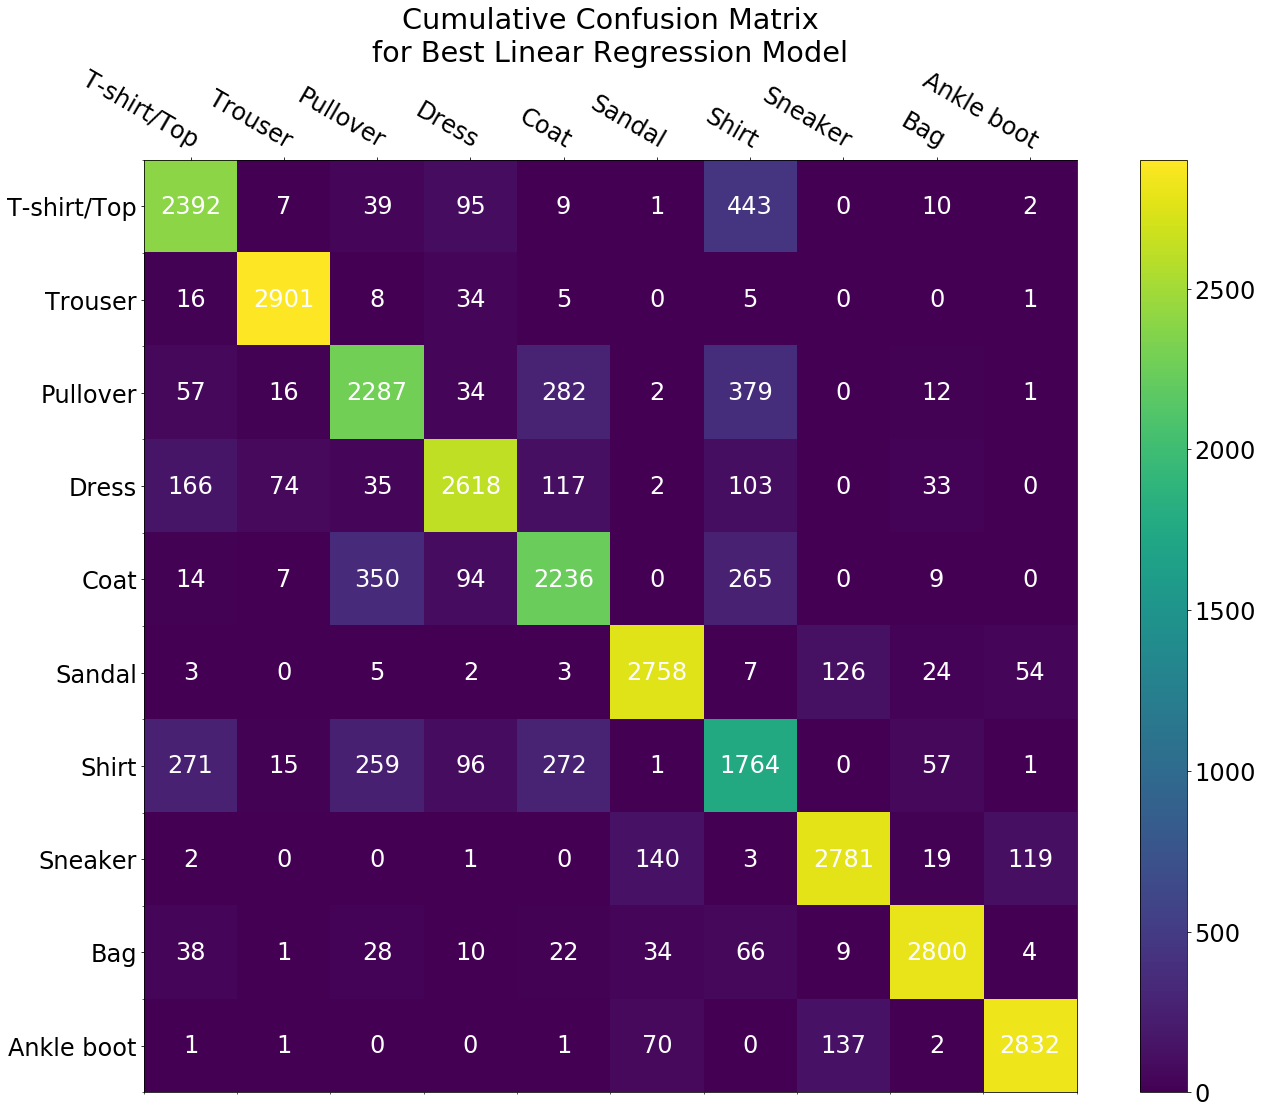
\includegraphics[width=0.7\textwidth]{img/conf_mat_lr.png}
    \caption{Cumulative confusion matrix across all folds for the best Binary Logistic Regression (One vs Rest) classifier.}
    \label{fig:conf_mat_lr}
\end{figure}

\pagebreak

\subsubsection*{Multinomial Logistic Regression}
\textbf{eta=0.05, epochs=250}
\begin{verbatim}
Mean training time: 54.3756s

Mean prediction time: 0.0256s

Mean Accuracy: 0.7982

Mean Precision:
[0.79839245 0.94701683 0.73793274 0.79150497 0.70485267 0.92682741
 0.60545925 0.87912836 0.91506139 0.91745585]

Mean Recall:
[0.71621622 0.95863113 0.60239599 0.83782631 0.69672086 0.89161794
 0.54597555 0.89908175 0.92010647 0.91178302]

Mean F1:
[0.74256119 0.952461   0.61258572 0.80815645 0.67354938 0.90837514
 0.50565056 0.88522393 0.91709617 0.91290083]
\end{verbatim}

\begin{figure}[H]
    \centering
    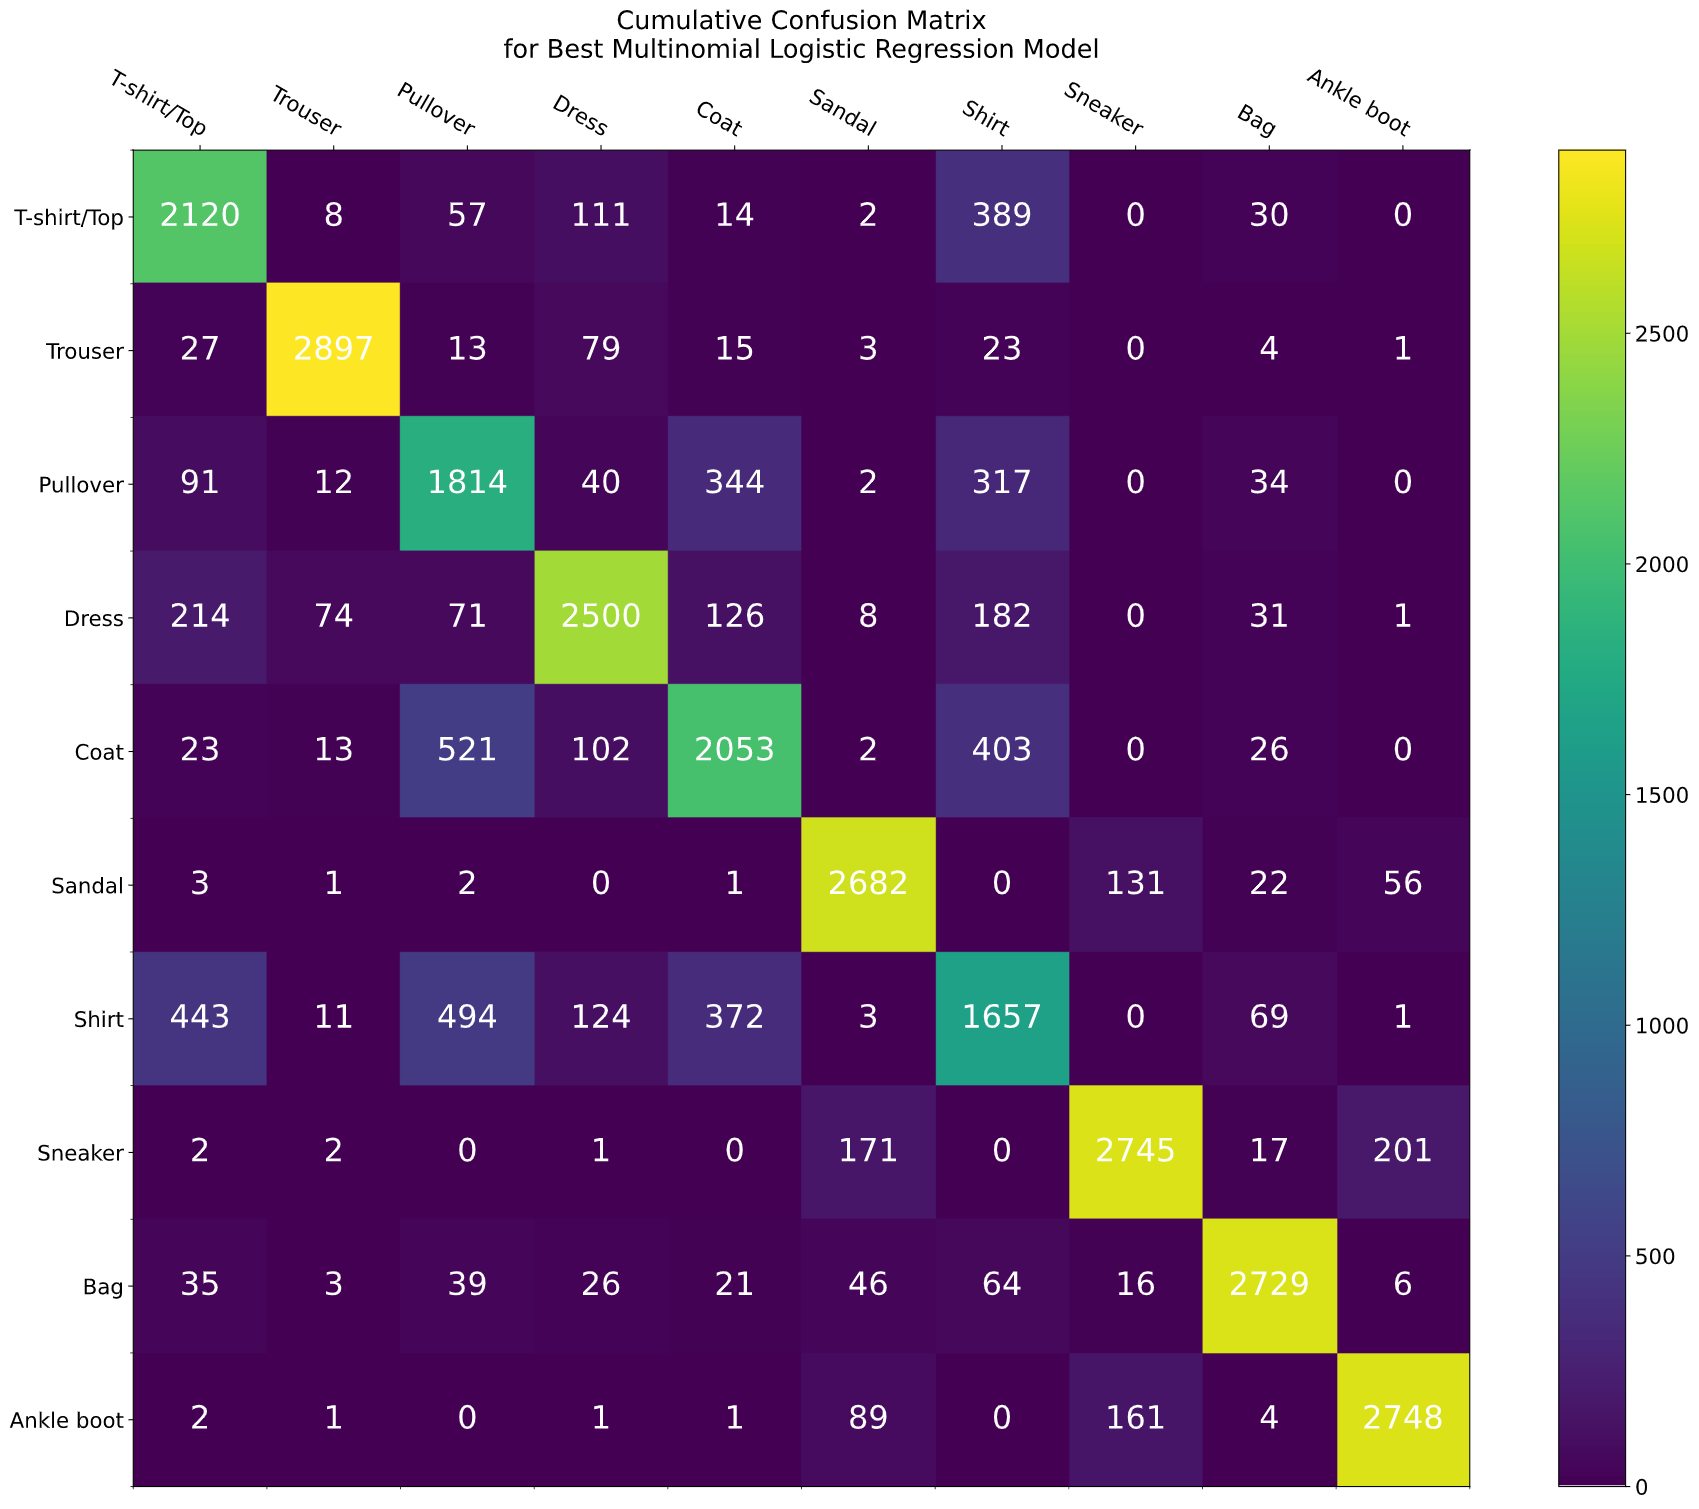
\includegraphics[width=0.7\textwidth]{img/conf_mat_mlr.png}
    \caption{Cumulative confusion matrix across all folds for the best Multinomial Logistic Regression classifier.}
    \label{fig:conf_mat_mlr}
\end{figure}

\pagebreak

\subsubsection*{Naive Bayes}
\textbf{laplace=1.0}
\begin{verbatim}
Mean training time: 0.3876s

Mean prediction time: 0.0198s

Mean Accuracy: 0.6664

Mean Precision:
[0.74157424 0.98229906 0.61906961 0.66011596 0.45564595 0.7376524
 0.33441587 0.58971677 0.88814489 0.69588295]

Mean Recall:
[0.79155405 0.89345398 0.59216849 0.88371417 0.63213536 0.15526024
 0.15321022 0.91549127 0.81593184 0.83545687]

Mean F1:
[0.76548335 0.93564555 0.60474426 0.75538131 0.5293982  0.25633562
 0.20990478 0.71726538 0.85029551 0.75918138]
\end{verbatim}

\begin{figure}[H]
    \centering
    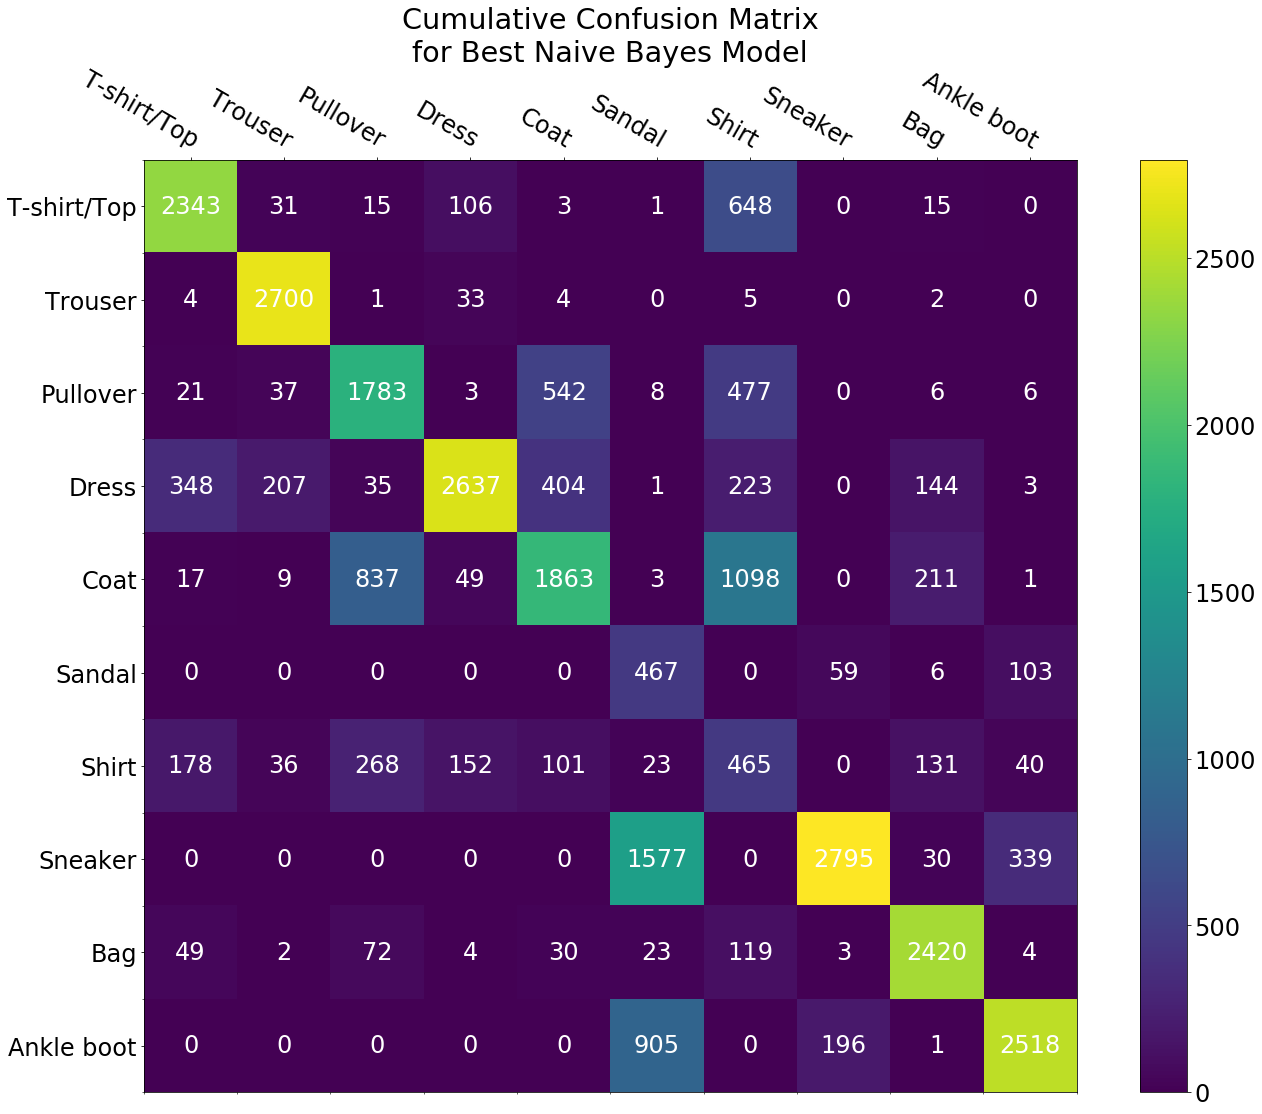
\includegraphics[width=0.7\textwidth]{img/conf_mat_nb.png}
    \caption{Cumulative confusion matrix across all folds for the best Naive Bayes classifier.}
    \label{fig:conf_mat_nb}
\end{figure}

\pagebreak

\subsubsection*{K-Nearest Neighbour}
\textbf{k=3, dist=manhattan}
\begin{verbatim}
Mean training time: 0.0003s

Mean prediction time: 148.2729s

Mean Accuracy: 0.8490

Mean Precision:
[0.74838203 0.98388233 0.70179857 0.89539027 0.7804547  0.98052861
 0.65385576 0.88746578 0.98078678 0.90433979]

Mean Recall:
[0.85608108 0.96426573 0.79275373 0.86695248 0.70884469 0.88131672
 0.58417904 0.93678024 0.94234917 0.95588766]

Mean F1:
[0.79846003 0.97393321 0.74402335 0.88074636 0.74275956 0.92818834
 0.61672485 0.91133918 0.96112016 0.9293543 ]
\end{verbatim}

\begin{figure}[H]
    \centering
    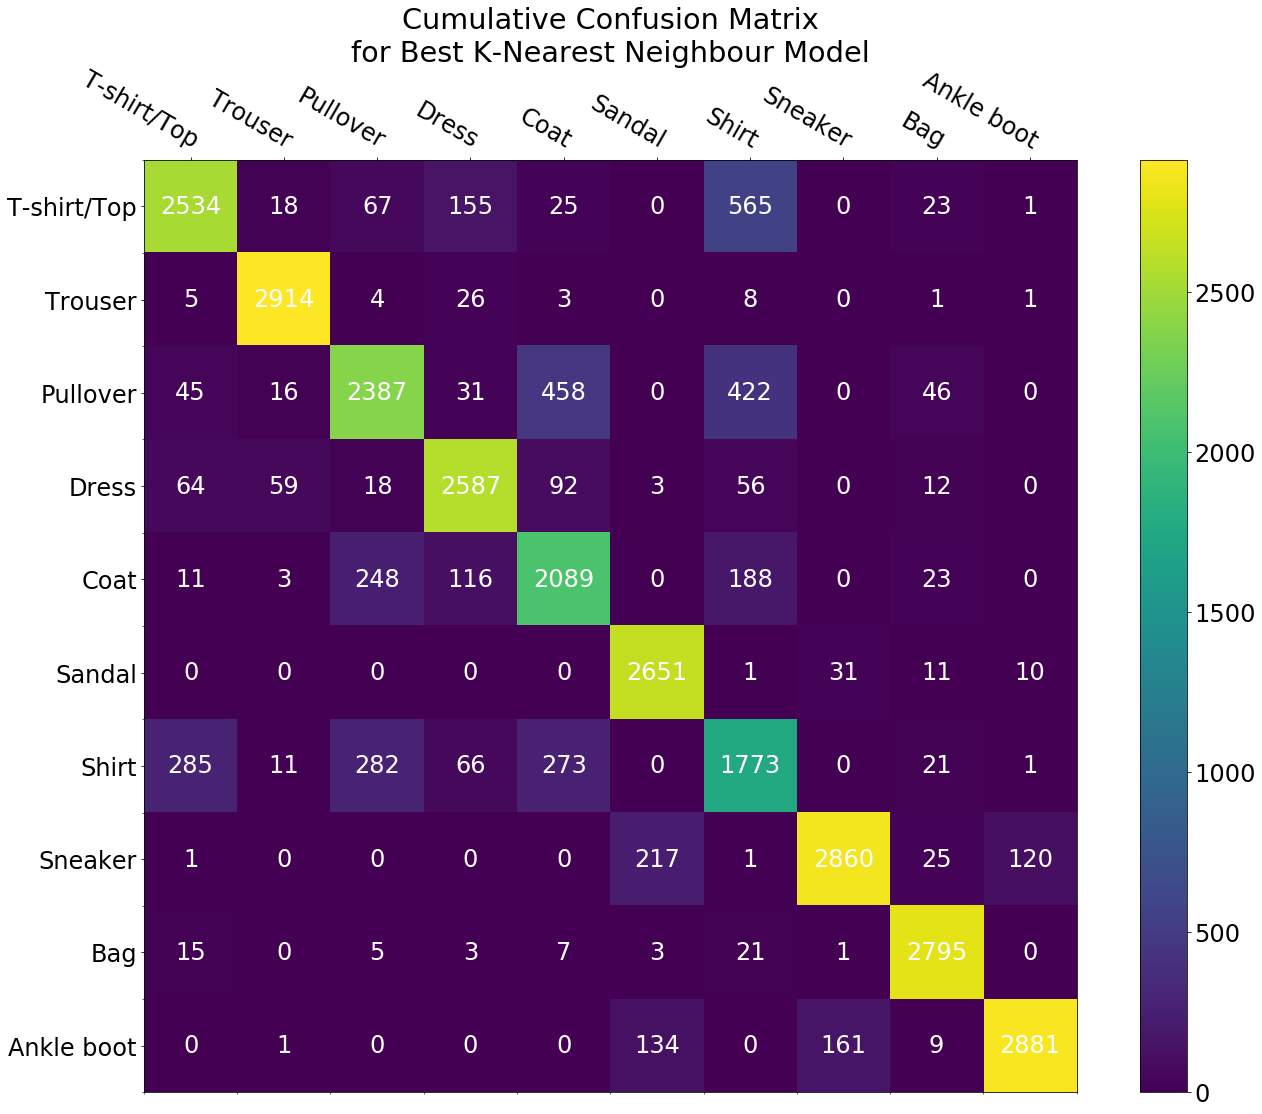
\includegraphics[width=0.7\textwidth]{img/conf_mat_knn.png}
    \caption{Cumulative confusion matrix across all folds for the best K-Nearest Neighbour classifier.}
    \label{fig:conf_mat_knn}
\end{figure}

\pagebreak

\subsubsection*{Neural Network}
\textbf{shape=(784, 100, 20, 10), activation=sigmoid, eta=0.05, batch\_size=64, epochs=250}
\begin{verbatim}
Mean training time: 171.4545s

Mean prediction time: 0.0589s

Mean Accuracy: 0.8550

Mean Precision:
[0.8017319  0.97504806 0.77303743 0.85552346 0.76848373 0.93091832
 0.65996621 0.91445806 0.94983404 0.92505939]

Mean Recall:
[0.79898649 0.96823924 0.770499   0.87465938 0.77196011 0.93052049
 0.64151902 0.90992393 0.94302257 0.93962289]

Mean F1:
[0.79982213 0.97161431 0.77121738 0.86451959 0.76796481 0.93068221
 0.64932603 0.91215338 0.94615582 0.9322106 ]

\end{verbatim}
\begin{figure}[H]
    \centering
    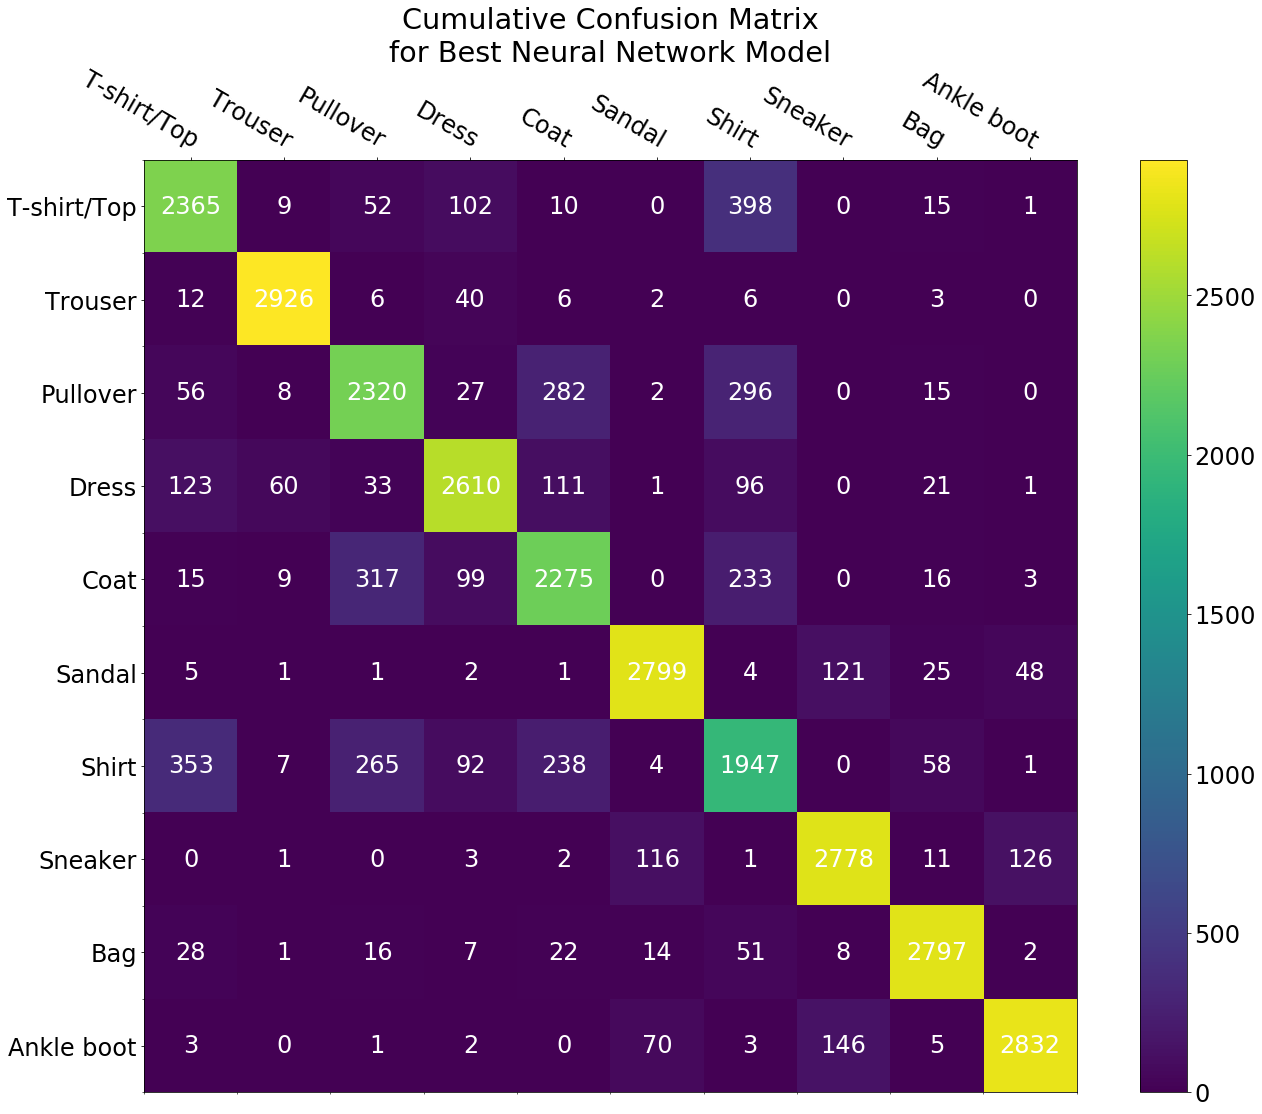
\includegraphics[width=0.7\textwidth]{img/conf_mat_nn.png}
    \caption{Cumulative confusion matrix across all folds for the best Neural Network classifier.}
    \label{fig:conf_mat_nn}
\end{figure}

\end{document}
